% !TeX spellcheck = en_GB
\documentclass[12pt,a4paper,oneside, titlepage]{article}

\usepackage[utf8]{inputenc}
\usepackage[T1]{fontenc}
\usepackage[french]{babel}
\usepackage{amssymb}
\usepackage{amsmath}
\usepackage{graphicx}
\usepackage{float}
\usepackage{url}
\usepackage{mathtools}
\usepackage{enumitem}
\setitemize{noitemsep,topsep=20pt,parsep=10pt,partopsep=0pt}
\setlist[enumerate]{label*=\arabic*.}
\usepackage{authblk}
\usepackage{hyperref}
\hypersetup{
    colorlinks=true,
    citecolor=black,
    linkcolor=black,
    urlcolor=black,
    linktoc=all
}
\usepackage[a4paper]{geometry}
\renewcommand{\familydefault}{\sfdefault}
\graphicspath{ {../../docs/} }
\newcommand{\todo}[1]{\par \textcolor{blue}{\textbf{To-Do $\mathbb{\to}$ #1}}\par}
\setcounter{tocdepth}{2}
\usepackage[font=small,labelfont=bf]{caption} % Required for specifying captions to tables and figures
\usepackage{booktabs}
\usepackage{tabularx}
\usepackage{arydshln}
\def\arraystretch{2.5}
\setlength\tabcolsep{20pt}

\newcommand{\rpm}{\raisebox{.2ex}{$\scriptstyle\pm$}}

\begin{document}
\renewcommand{\labelitemi}{$\bullet$}
\setlength\parindent{0pt}

\section*{Chapitre 3 : Réseaux d’interconnexion}

  \section*{Définition}

    \begin{itemize}
      \item Ordinateur parallèle = processeurs + mémoires + \textbf{réseau d'interconnexion}
      \item Ce réseau permet la communication entre les unités de traitement.
      \item $\implies$ besoin d'interconnexion rapide et fiable.
    \end{itemize}

  \subsection*{Topologie}

    \begin{itemize}
      \item Pas possible d'interconnecter tout les processeurs (prix)
      \item \textbf{Topologie} = structure des liens entre les processeurs
      \item Processeurs = adjacents si reliés par une connexion directe
      \item Processeurs = distants si nécessaire de passer par des procs intermédiaires
      \item Le ràseau peut être vu comme un graph ou :
      \begin{itemize}
        \item noeud = processeur ou mémoire
        \item arc = connexion (bidirectionelle ou non)
      \end{itemize}
      \item Topologie statique = connexions fixes
      \item Topologie dynamique = possibilité de reconfigurer les connexions
    \end{itemize}

    \subsubsection*{Performances d'un réseau}

      \paragraph{Diamètre} D = longueure du chemin le plus court entre les 2 noeuds les plus éloignés

      \paragraph{Connectivité} Nombre de noeuds adjacents à chaque noeuds (= \textbf{Degré})

      \paragraph{Latence} Temps nécessaire à un message pour transiter entre les 2 noeuds les plus éloignés.
      Dépends du diamètre et de la technologie utilisé (+ préparation du message et correction d'erreurs)

      \paragraph{Bandwidth} Débit d'information qu'un noed peut transmettre dans le réseau (généralement MByte/s)

      \paragraph{Largeur bisectionnelle} Nombre d'interconnexions entre deux moitiés identiques d'un réseau (fig 3.1 p 58).
      Si il existe plusieurs façon de diviser le réseau on prends la plus défavorable.

      \paragraph{Scalabilité} Possibilité d’augmenter la taille du réseau en ajoutant des processeurs

      \paragraph{Prix} Nombre decomposants en fonction du nombre de noeuds

      \paragraph{Fonctionnalité}  Capacité de combiner des messages allant vers une même destination et gestion des conflits de routage

      \paragraph{Capacité} Nombre de messages mximum simultanés dans le réseau

    \subsection*{Le routage}

      \begin{itemize}
        \item \textbf{Routage} = algorithme de transite d'un message le plus efficacement possible entre les noeuds dans un réseau donné
        \item Routage minimal = chemins les plus courts entre la source et la destination
        \item Routeur = circuit chargé du routage
        \item L'algorithme de routage doit éviter :
        \begin{itemize}
          \item Deadlock = message bloqué de façon indéfinie
          \item Livelock = message tournant en boucle sans arriver à destination
        \end{itemize}
        \item Single-port (\textit{processor bound}) = communication n’utilisant qu’un seul canal à la fois
        \item Multi-port (\textit{link bound}) = communication utilisant plusieurs canaux simultanément
        \item Routage local = les noeuds acheminnent les message uniquement en se basant sur une information locale
        \begin{itemize}
          \item Routage local déterministe = information locale = adresse de destination du message
          \item Routage local adaptif = information sur le reste du réseau (chemins de taille similaire, pannes)
        \end{itemize}
        \item Routage synchrone = messages envoyés simultanéments et sousmis à un cycle de routage complet (temps de transfert = celui du message le plus lent)
        \item Routage asynchrone = messages envoyés et reçu en fonctions des besoins du programme
      \end{itemize}

      \subsection*{Primitives de communication}

      \begin{itemize}
        \item Point à point (one to one)
        \item Permutation
        \item Broadcast (one to all)
        \item Réduction (many to one)
        \item Echange total (all to all)
        \item Distribution (one to all personalisé) = envoi de message différents à tout les noeuds (par ex Scatterv en MPI)
        \item Gather = inverse de Scatter (all to one personalisé)
        \item Echange total personalisé = tout les processeurs envoient un message différents à tout les autres processeurs
        \item Scans = calcule de la donnée finale en fonction des données précédents (noeuds 1 à $i-1$)
      \end{itemize}


      \subsection*{Technique de dommunication}

      \begin{itemize}
        \item \textbf{Store and forward} = envoi du message du noeud $i-1$ au noeud $i$ (stockage dans $i$), ensuite envoi de $i$ à $i+1$
        \begin{itemize}
          \item Temps de transfert du message proportionel à la bandwidth, la longueur du message et le nombre de noeuds + temps de préparation du message
          \item $t_{sf}=t_{s} + L (n - 1) \frac{1}{W}$
          \item Pas rapide (n'exploite pas la puissance du réseau)
        \end{itemize}
        \item \textbf{Cut through} = Les messages peuvent continuer sans être reçu complètement par un noeud
        \item \textbf{Wormhole} est un exemple de Cut through
        \begin{itemize}
          \item Découpe du message en morceaux de taille fixe (flit)
          \item Seul le premier flit contient l'adresse
          \item Tout les flits suivants suivent le premier (comme des wagons avec une locomotive)
          \item $t_{wh} = t_{s} + (n - 1 + L - 1) \frac{1}{W}$
          \item Beaucoup plus efficace que Store and forward
        \end{itemize}
        \item Canaux virtuels = mutiplexage en temps du canal physique pour éviter les deadlocks
      \end{itemize}

  \section*{Réseaux statiques}

    Réseaux avec connexions physiques fixes entre les noeuds $\implies$ impossible de modifier la topologie.

    \subsection*{Anneaux et chaînes}

    \begin{figure}[H]
      \centering
      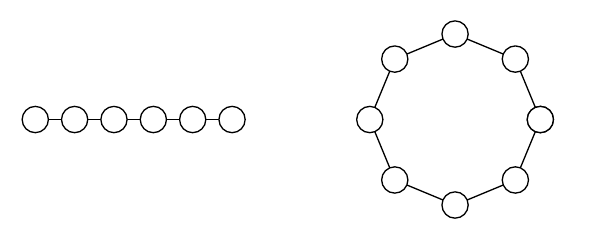
\includegraphics[width=0.75\textwidth]{images/linAnneau}
      \caption{Topologie Linéaire et en Anneau}
    \end{figure}

    \begin{itemize}
      \item Adapté au traitement de problèmes unidimensionnels
      \item Diamètre : $D = N/2$
      \item largeur bisectionnelle = 2
      \item Prix = $\sim N$
    \end{itemize}

    \subsection*{Grilles de processeurs (mesh)}

    \begin{figure}[H]
      \centering
      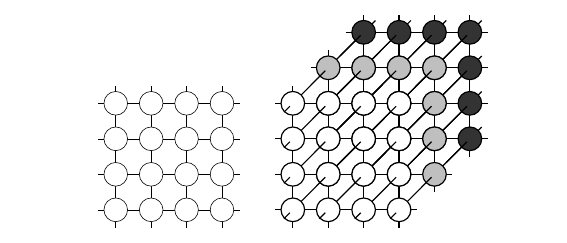
\includegraphics[width=0.75\textwidth]{images/mesh}
      \caption{Topologie en grille (2D et 3D)}
    \end{figure}

    \begin{itemize}
      \item Mesh 2D plus répandus (ILLIAC, IV, DAP, Paragon)
      \item Mesh 3D : T3E, Parsytec
      \item Diamètre : $D = d N^{1/d}$ avec $d$ la dimension
      \item Si les bords sont reliés $D = \frac{1}{2} d N^{1/d}$
      \item Le prix est proportionel à $N$
      \item Le routage s'effectue le long des axes de la grille
      \item Risque de congestion avec un routage X-Y
      \item Broadcast par ligne et ensuite colones par exemple $O(\sqrt{N})$ (fig 3.8)
    \end{itemize}

    \subsection*{hypercube}

      \begin{figure}[H]subsection name
        \centering
        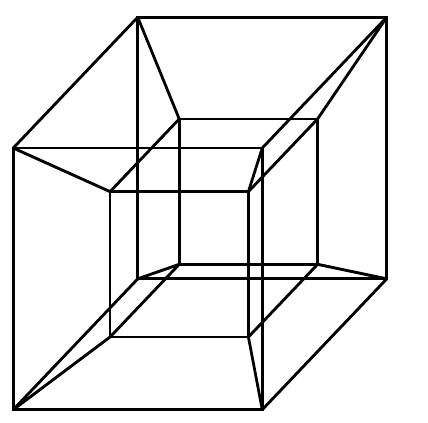
\includegraphics[width=0.5\textwidth]{images/hyp}
        \caption{Topologie hypercube de degré 4}
      \end{figure}

      \begin{itemize}
        \item Généralisation du cube dans une dimension supérieur à 3
        \item Pour $k$ dimensions et des bords de longueur 2 on aura $2^k$ noeuds
        \item Chaque noeuds est de degré $k$ ($k$ voisins)
        \item Diamètre $D = k$
        \item Le nombre de chemins entre deux noeuds augmente avec la taille de l'hypercude $\implies$ moins de risques de congestion
        \item Routage dans un réseau hypercubique :
        \begin{itemize}
          \item Numérotation des noeuds en binaire ($k$ bits)
          \item Les noeuds reliés le long de la dimension $l$ diffèrent que du $l$ ième bit
          \item Pour aller de entre 2 noeuds (adresse $A$) on fait $A_1 \oplus A_2$ pour obtenir le vecteur
        \end{itemize}
        \item Broadcast en hypercube : Connexion multiport (one to many), la racine envoi dans toute les dimensions $i$ puis chaque noeuds envois dans les dimensions inférieurs à $i$
        \item Echange total hypercubique : Chaque noeud envois ses données plus toutes celles reçue précédément dans la dimension $l$ le tout $N-1$ fois
        \item Pour mapper une grille sur un hypercube on utilise la fonction de Gray
      \end{itemize}

    \subsection*{Arbres binaires}

      \begin{figure}[H]subsection name
        \centering
        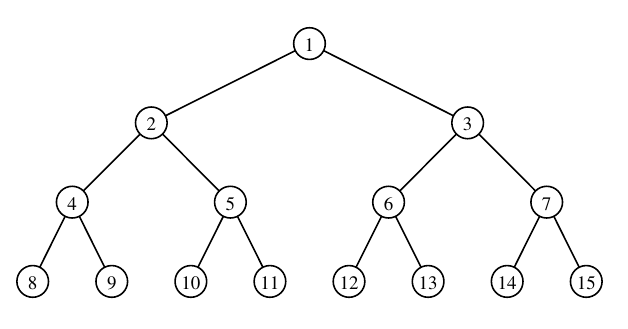
\includegraphics[width=0.5\textwidth]{images/tree}
        \caption{Topologie Arbre binaire}
      \end{figure}

      \begin{itemize}
        \item Topologie relativement peu utilisée dans sa forme statique
        \item Divisé en $k$ niveaux ($l$) avec $2^l$ noeuds
        \item Nombre de noeuds = $2^{k + 1}-1$
        \item Diamètre : $D = 2k$
        \item degré des noeuds = 3 sauf aux extrémité
        \item Largeure bisectionnelle = 1 $\implies$ bottleneck
        \item Scallable proportionellement à $N$
        \item Routage : en représentant les numéros de noeuds sous forme binaire on remonte au parent commun (prefix binaire similaire)
      \end{itemize}

    \subsection*{Réseaux de permutation et “shuffle exchange”}

      \begin{itemize}
        \item Utilisation de fonctions de permutations bijectives plutôt que des représentations géométriques
        \item 2 noeuds $i$ et $j$ sont reliés si $f(i)=j$
        \item \textbf{Perfect shuffle} : décalage des bits vers la droite ($010 \rightarrow 001$)
        \item \textbf{Inverse shuffle} : décalage des bits vers la gauche ($010 \rightarrow 100$)
        \item \textbf{Butterfly} : échange du premier et dernier bit ($100 \rightarrow 001$)
        \item \textbf{Bit reversal} : inversion de l'ordre des bits ($0100 \rightarrow 0010$)
        \item \textbf{Exchange} : remplacement du bit de poid faible par son complément à 1 ($0111 \rightarrow 0110$)
        \item Important de combiner deux opération si pas cyclique
        \item "Shuffle exchange" = combinaison de shuffle et exchange (no shit)
        \begin{itemize}
          \item Degré : $D = 3$
          \item Prix = $3N$
          \item Scalabilité compliqué car si $N++$ les connexions changent

        \end{itemize}
      \end{itemize}

\end{document}
